%%%%%%%%%%%%%%%%%%%%%%%%%%%%%%%%%%%%%%%%%%%%%%%%%%%%%%%%%%%%%%%%%%%%%%%%%%%%%%
\documentclass[12pt,hidelinks]{article}

% 1. Load LaTeX packages
\usepackage{fontspec}
\usepackage{geometry}
\usepackage{lastpage}
\usepackage{fancyhdr}
\usepackage{hyperref}
\usepackage{amsmath}
\usepackage{amsthm}
\usepackage{xunicode}
\usepackage{listings}
\usepackage{color}
\usepackage{amssymb}

% 2. Define page dimensions and spacing
\geometry{top=1in, bottom=1in, left=1in, right=2in, marginparsep=4pt,
          marginparwidth=1in}
\setlength{\parindent}{0pt}
\setlength{\parskip}{12pt}

% 3. Set header, footer, and bibliography
\renewcommand{\headrulewidth}{0pt}
\pagestyle{fancyplain}
\fancyhf{}
\lfoot{}
\rfoot{page \thepage\ of \pageref{LastPage}}
\bibliographystyle{acm}

% 4. Set fonts for the document
\defaultfontfeatures{Mapping=tex-text}
\setromanfont{YaleNew}

% 5. Define custom code for book environments and commands
\DeclareMathOperator*{\argmin}{arg\,min}
\DeclareMathOperator*{\argmax}{arg\,max}
\newcommand{\code}[1]{\texttt{#1}}
\newcommand{\pkg}[1]{\textbf{#1}}

% 6. Define custom code for book environments and commands
\definecolor{verbgray}{gray}{0.9}
\definecolor{verbgray2}{gray}{0.975}

\lstnewenvironment{rcode}{%
  \lstset{backgroundcolor=\color{verbgray},
  frame=single,
  framerule=0pt,
  basicstyle=\ttfamily,
  keepspaces=true,
  columns=fullflexible}}{}

\lstnewenvironment{rres}{%
  \lstset{backgroundcolor=\color{verbgray2},
  frame=single,
  framerule=0pt,
  basicstyle=\ttfamily,
  keepspaces=true,
  columns=fullflexible}}{}

% 7. Define numbering scheme for equations (only needed for handout).
\numberwithin{equation}{section}
\setcounter{section}{5}

%%%%%%%%%%%%%%%%%%%%%%%%%%%%%%%%%%%%%%%%%%%%%%%%%%%%%%%%%%%%%%%%%%%%%%%%%%%%%%
\begin{document}

{\LARGE Handout 05: Expectation and Variance}

\vspace*{18pt}

This class does not require that you have had any prior probability theory
and we certainly do not have time to discuss and derive all of the details
that would be covered in a semester of MATH329. However, it will be very
useful to complete our study of linear regression and to motivate the next
steps if we can use some probability theory. The notes here lay out the basic
points about random variables, expected values, and variance.

\textbf{Random variables}

A random variable provides, conceptually, a way of representing uncertainty
in a value. Instead of the fixed value (albeit often unknown) we typically
denote with a variable such as $x$, a random variable has information about
all of the possible outcomes it might take on and the chance that it takes
on one of those values. It is possible to derive a more general theory, but
today we will restrict ourselves to the case of random variables that take on
real valued quantities.

The mathematical definition of a random variable $Z$ (in our restricted case)
is given by a function $f(z)$---the \textit{density function}---that maps the
real line into the unit interval and has an integral of $1$:
\begin{align}
f: \mathbb{R} \rightarrow [0, 1] \\
\int_{-\infty}^{+\infty} f(z) dz = 1.
\end{align}
How does this object represent randomness? We define the probability that the
random variable is between two value $a$ and $b$ as the integral of the function
between these two values.
\begin{align}
Pr(a \leq Z \leq b) &= \int_a^b f(z) dz
\end{align}
You can see now why we force the total integral to be one: the random variable
has to be somewhere.

The expected value of a random variable describes the equivalent of the mean
of the random variable. We can define the expected value as:
\begin{align}
\mathbb{E} Z = \int_{-\infty}^{+\infty} z\cdot f(z) dz.
\end{align}
You should convince yourself that this makes sense, for example by considering
a random variable with a function $f$ that is symmetric around the origin (it
should have an expected value of $0$, at least as long as the integral
converges).

The expected value tells us where the center of the random variable is. The
variance tells us how much a random variable varies around this center.
Specifically, the variance is the expected squared value of the distance a
random variable will be away from its mean. Or, symbolically:
\begin{align}
\mathbb{V}ar(Z) &= \mathbb{E} \left[ \left(Z - \mathbb{E} Z \right)^2 \right]
\end{align}
Whenever possible, when working with expected values and variances, you will
want to avoid go back to the original definitions.  We will ultimately need
vector version of these two operators, but to avoid moving too quickly here
are some basic properties of the expected value and variance. Let $Z$ be a random
variable and $a$ be a non-random variables. Then:
\begin{align}
\mathbb{E}(aZ) &= a \cdot \mathbb{E}(Z) \\
\mathbb{E}(a + Z) &= a + \mathbb{E}(Z) \\
\mathbb{V}ar(aZ) &= a^2 \cdot \mathbb{V}ar(Z) \\
\mathbb{V}ar(a + Z) &= \mathbb{V}ar(Z)
\end{align}
It is much better---conceptually and theoretically---to treat these as
operators that have particular properties.

\begin{figure}
\begin{center}
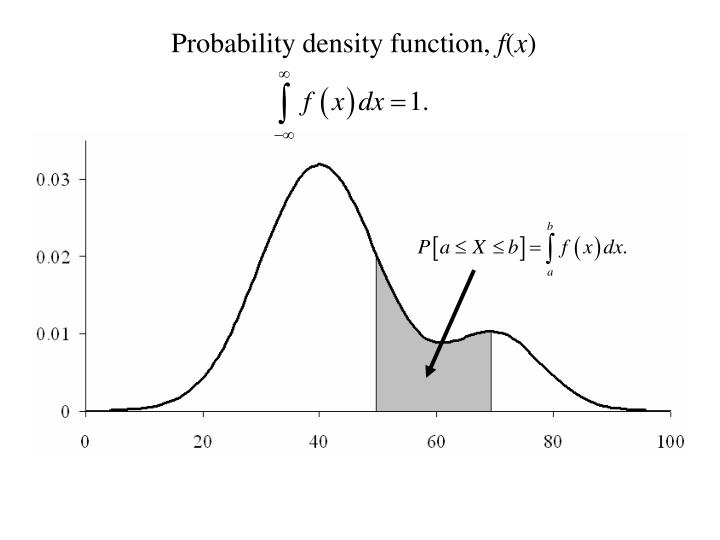
\includegraphics[width=\textwidth]{figures/pdensfun.jpg}
\end{center}
\caption{Example of a probability density function.}
\end{figure}

\textbf{Random vectors}

To actually make use of the probability theory given here in the theory of
linear regression, we need to extend our definitions to random vectors. A random
vector $\epsilon$ is just a vector where each component $\epsilon_i$ is itself
a random variable:
\begin{align}
\epsilon &= \begin{bmatrix} \epsilon_1 \\ \vdots \\ \epsilon_n \end{bmatrix}.
\end{align}
And the expected value of a random vector is the vector of expected values of
each component:
\begin{align}
\mathbb{E}\epsilon &= \begin{bmatrix} \mathbb{E}\epsilon_1 \\ \vdots \\ \mathbb{E}\epsilon_n \end{bmatrix}.
\end{align}
The variance of a random variable is a bit more involved. The variance is
given by an $n$-by-$n$ matrix, the diagonal of which is a variance of each
component. The off-diagonal quantities give the \textit{covariance} of the
respective components. Specifically:
\begin{align}
\mathbb{V}ar(\epsilon)_{i,j} &= \mathbb{E} \left[ \left(\epsilon_i - \mathbb{E} \epsilon_i \right)
\cdot \left(\epsilon_j - \mathbb{E} \epsilon_j \right) \right].
\end{align}
Two variables that have a covariance of zero are said to be \textit{uncorrelated}.
The entire variance matrix can be written compactly using the transpose operator:
\begin{align}
\mathbb{V}ar(\epsilon) &= \mathbb{E} \left[ \left(\epsilon - \mathbb{E} \epsilon \right)
\cdot \left(\epsilon - \mathbb{E} \epsilon \right)^t \right].
\end{align}
It is the formula that will be most helpful for us next week as we investigate
statistical learning extensions of the linear model.

It should be straightforward to see that the expected value of a vector equation
behaves similarly to the scalar version. Let $\epsilon$ be a random vector,
$v$ a non-random vector, and $A$ a non-random matrix. Then:
\begin{align}
\mathbb{E}(A \cdot \epsilon) &= A \cdot \mathbb{E}\epsilon \\
\mathbb{E}(v + \epsilon) &= v + \mathbb{E}\epsilon
\end{align}
There are also two equivalent properties for the Variance operator:
\begin{align}
\mathbb{V}ar(v + \epsilon) &= \mathbb{V}ar(\epsilon)\\
\mathbb{V}ar(A\epsilon) &= A \cdot \mathbb{V}ar(\epsilon) \cdot A^t
\end{align}
You will derive the last equations in today's lab.

%%%%%%%%%%%%%%%%%%%%%%%%%%%%%%%%%%%%%%%%%%%%%%%%%%%%%%%%%%%%%%%%%%%%%%%%%%%%%%
\newpage

\textbf{LAB QUESTIONS}

\vspace*{0pt}

\begin{enumerate}
\item Assume that $Z$ is a random variable that only takes values between $0$
and $5$. Any value in this range is equally likely to occur. Write down the
formula for the density function $f$ that corresponds to this random variable.
\item Without doing any calculations, what do you expect to be the expected
value of $Z$ in the previous question?
\item Using the formulae in the notes, show that your guess matches the mathematical
definition of $\mathbb{E}Z$.
\item Prove the equation given for $\mathbb{V}ar(AZ)$.
\item Assume that we have a random variable $y$ defined in terms of a random
variable $\epsilon$ such that:
\begin{align}
y &= X b + \epsilon.
\end{align}
Further assume that the expected value of the $\epsilon$ term is the zero vector
(a vector with zeros in every component). Show that the expected value of the
ordinary least squares equation for the estimate $\beta$ is equal to $b$.
This means that $\beta$ is an \textit{unbiased} estimator of $b$.
\item Using the same set-up as above, further assume that:
\begin{align}
\mathbb{V}ar(\epsilon) &= \sigma^2 \cdot I_n.
\end{align}
For some fixed value $\sigma^2 > 0$. What is the variance of $y$?
\item Finally, derive a formula for the variance of the ordinary least squares estimate $\beta$.
\end{enumerate}

\end{document}

